%!TEX root = ../../dissertation.tex
\chapter{Supporting Information}
\label{AppendixA}

The following figures reproduce the Supporting Information of Anand et al.\cite{anand2026improving}
in its published order, S1--S13. They support the sampling and system-preparation
results in Chapter~\ref{ch:benchmarking-and-system-preparation}, the resolvation
analysis in Chapter~\ref{ch:binding-pocket-resolvation}, and the conformational
analysis in Chapter~\ref{ch:apo-state-conformational-changes}.

\begin{figure}[htbp]
  \centering
  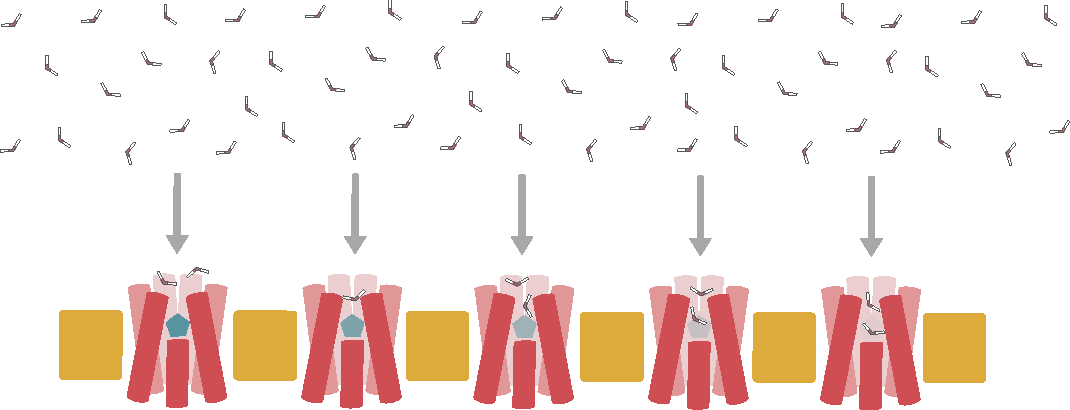
\includegraphics[width=\textwidth,height=0.56\textheight,keepaspectratio]{chapters/appendixA/figures/si_s1/si_figure_S1.pdf}
  \caption[GCMC-like binding-pocket resolvation scheme.]{Schematic of the GCMC-like process used to resolvate the protein binding pocket in ABFE windows approaching complete ligand annihilation. Fewer water molecules enter a pocket occupied by an interacting ligand (left); more water molecules can be inserted when the ligand is fully decoupled (right).}
  \label{fig:si-gcmc-schematic}
  \caption*{Reproduced from SI Figure S1 of Anand et al.\cite{anand2026improving} under CC BY 4.0.}
\end{figure}
\clearpage



\begin{figure}[p]
  \centering
  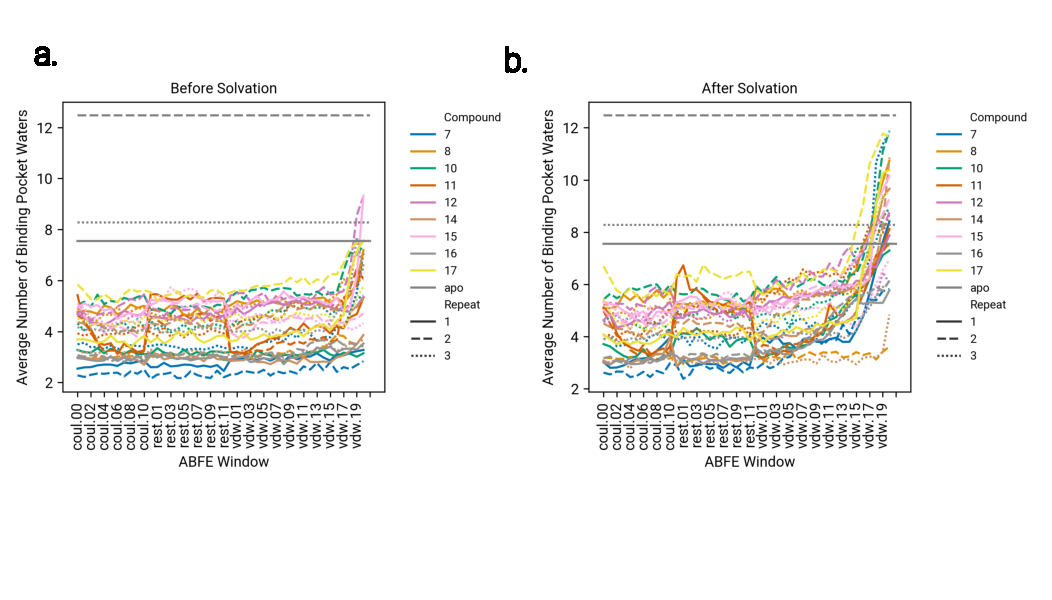
\includegraphics[width=\textwidth]{chapters/appendixA/figures/si_s3/si_figure_S3.pdf}
  \caption[mGlu5 water occupancy for additional compounds.]{Water occupancy across ABFE windows for the additional mGlu5 compounds, (a) before and (b) after the solvation step. Most compounds reach apo-level solvation in the final van der Waals decoupling leg after applying the solvation scheme.}
  \label{fig:si-mglu5-water-occupancy}
  \caption*{Reproduced from SI Figure S3 of Anand et al.\cite{anand2026improving} under CC BY 4.0.}
\end{figure}
\clearpage

\begin{figure}[p]
  \centering
  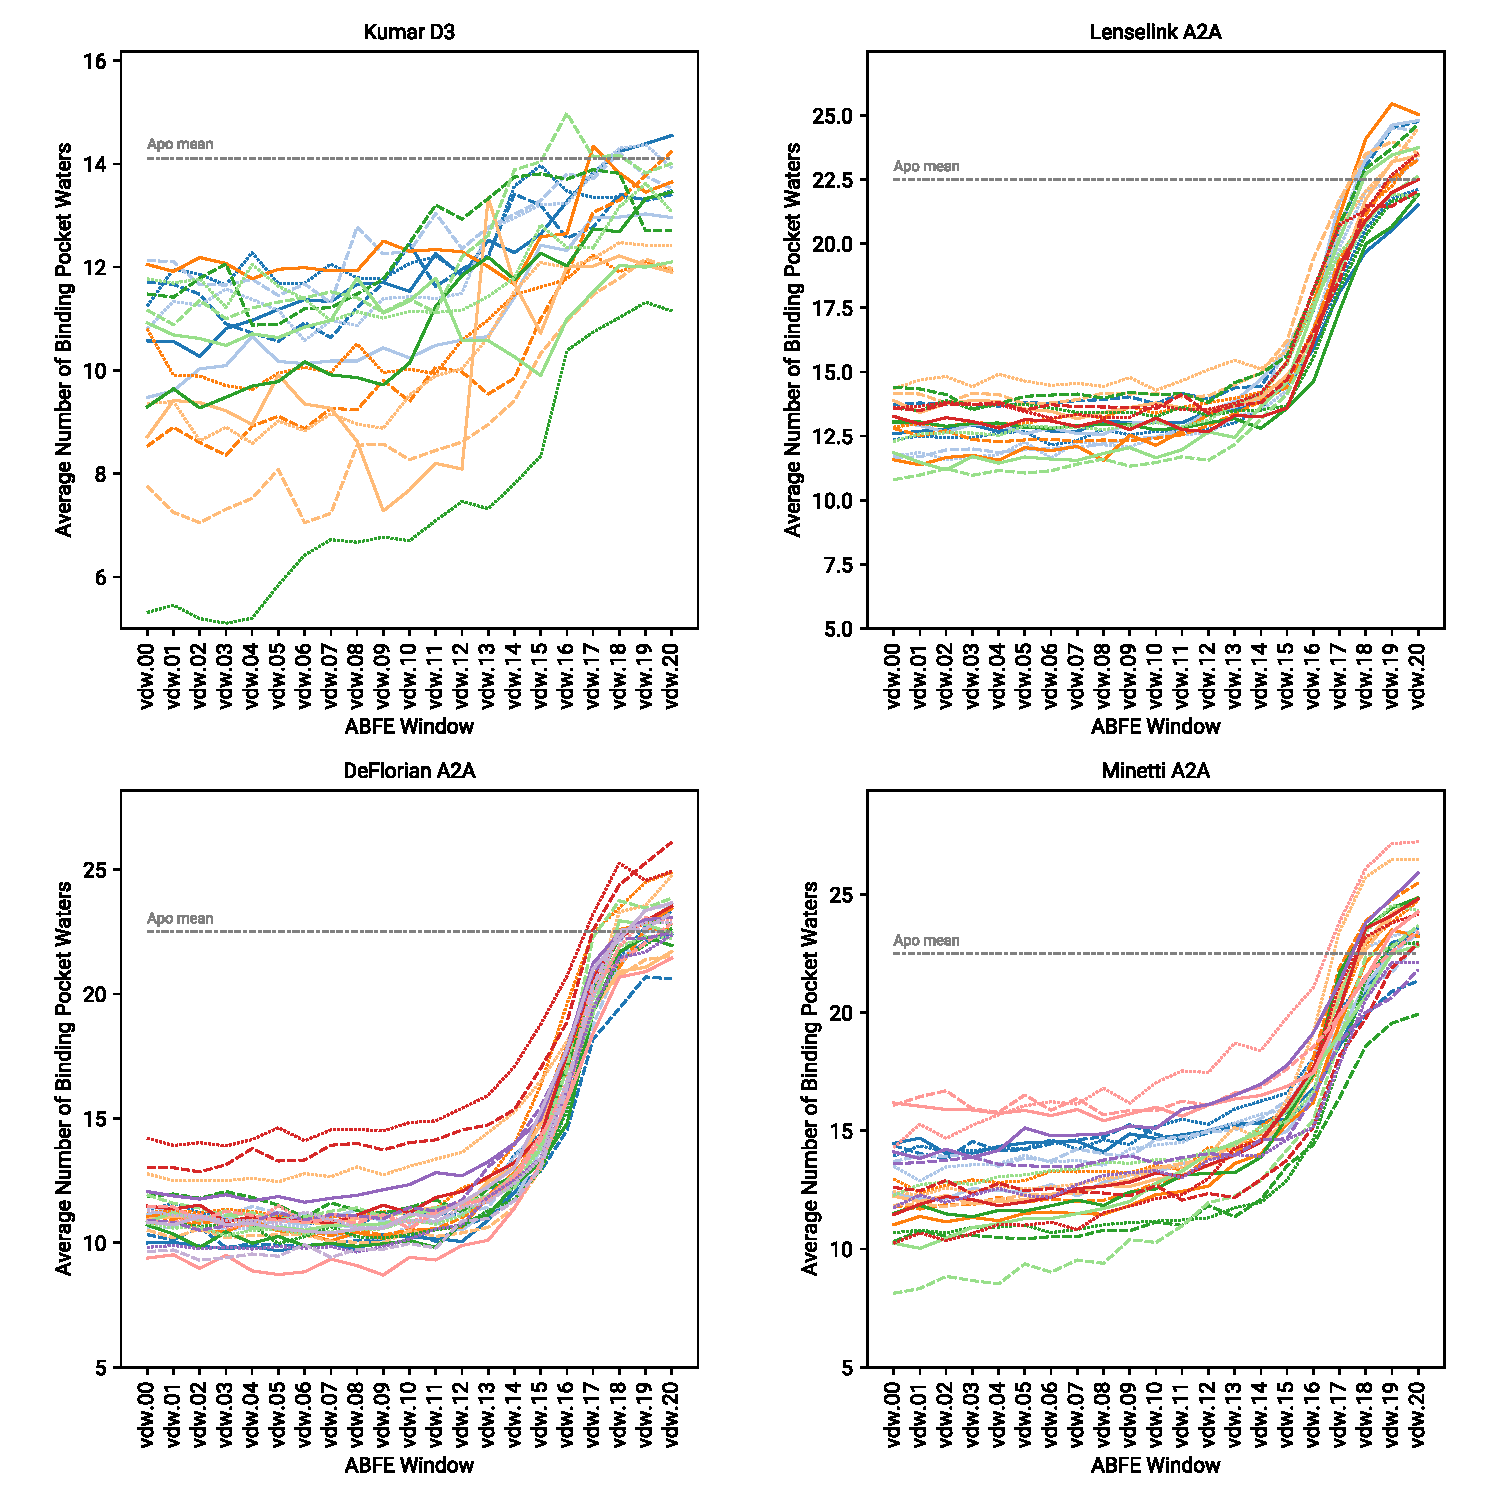
\includegraphics[width=\textwidth,height=0.68\textheight,keepaspectratio]{chapters/appendixA/figures/si_s4/si_figure_S4.pdf}
  \caption[Binding-pocket water occupancy across the class A GPCR datasets.]{Binding-pocket water occupancy across the van der Waals decoupling windows for the Kumar D3, Lenselink A$_{2A}$, Deflorian A$_{2A}$, and Minetti A$_{2A}$ datasets. Colours identify ligands and line styles identify independent ABFE repeats. Grey horizontal lines show the apo binding-pocket water-occupancy reference.}
  \label{fig:si-all-datasets-water-occupancy}
  \caption*{Reproduced from SI Figure S4 of Anand et al.\cite{anand2026improving} under CC BY 4.0.}
\end{figure}
\clearpage

\begin{figure}[p]
  \centering
  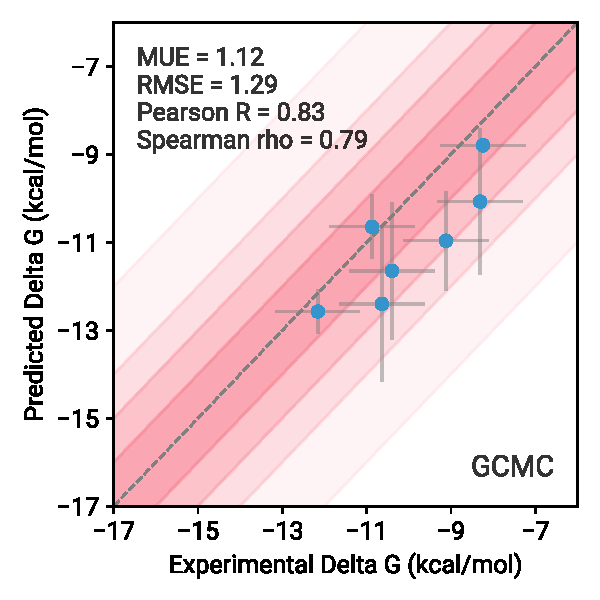
\includegraphics[width=0.80\textwidth,height=0.60\textheight,keepaspectratio]{chapters/appendixA/figures/si_s5/si_figure_S5.pdf}
  \caption[Lenselink ABFE predictions with GCMC-like resolvation.]{Experimental and predicted binding free energies for the Lenselink dataset with GCMC-like resolvation. Error bars show the standard deviation across starts. Shaded diagonal bands indicate deviations of $1$, $2$, $3$, and $5\,\mathrm{kcal\,mol^{-1}}$ from perfect agreement.}
  \label{fig:si-lenselink-gcmc}
  \caption*{Reproduced from SI Figure S5 of Anand et al.\cite{anand2026improving} under CC BY 4.0.}
\end{figure}
\clearpage

\begin{landscape}
\begin{figure}[p]
  \centering
  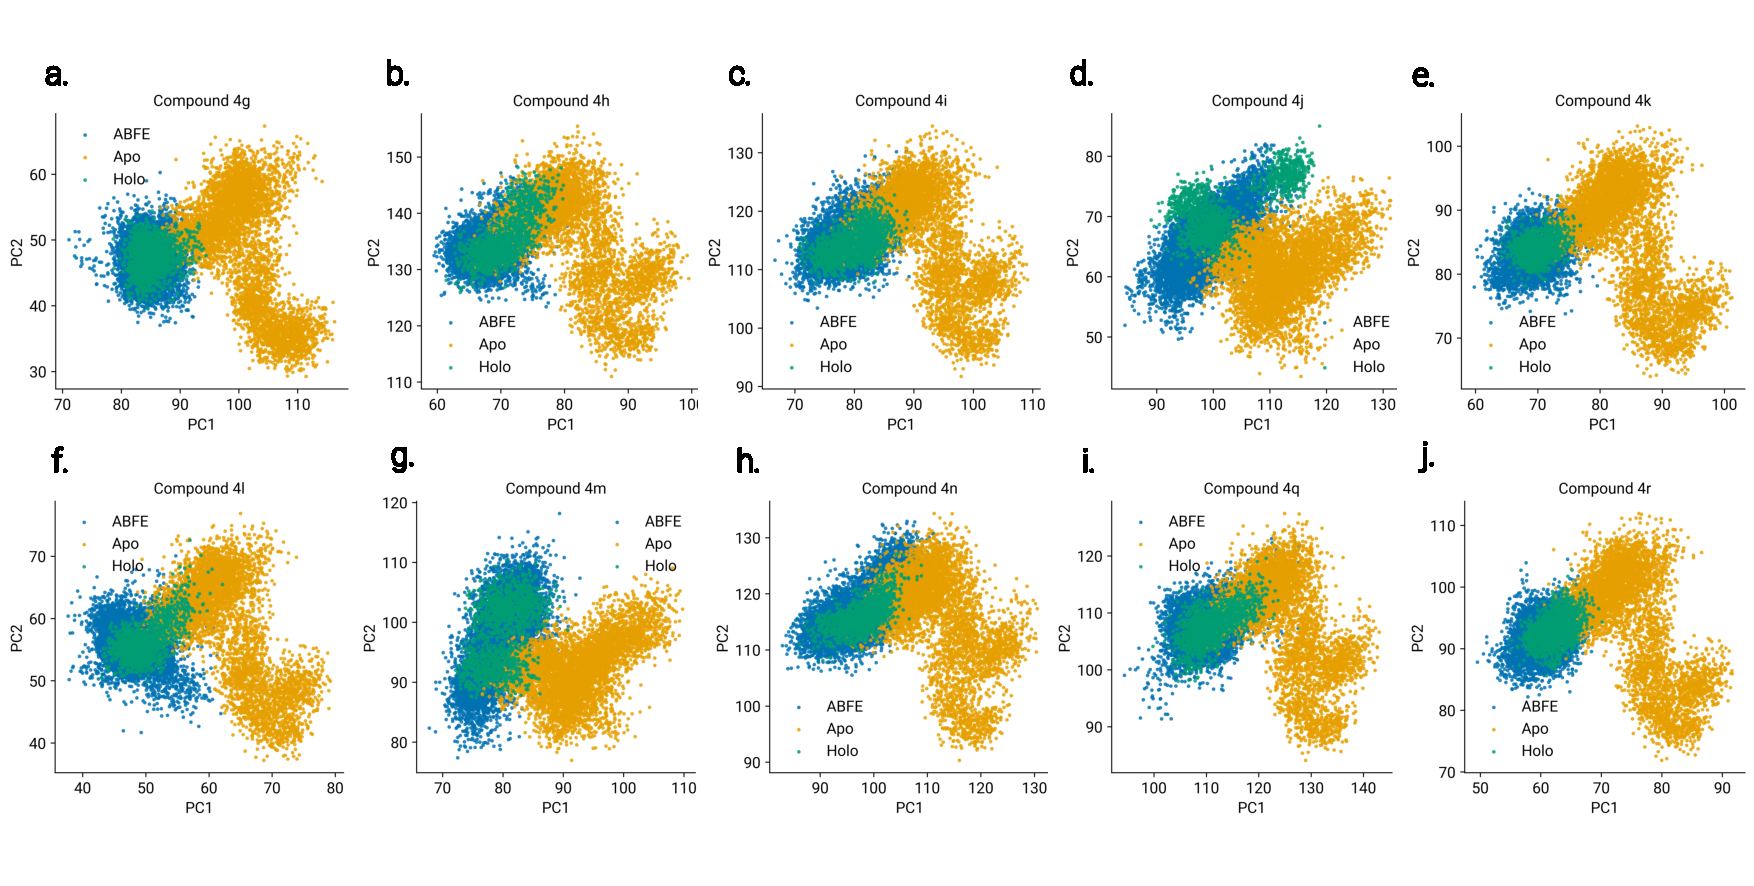
\includegraphics[width=\linewidth,height=0.68\textheight,keepaspectratio]{chapters/appendixA/figures/si_s6/si_figure_S6.pdf}
  \caption[Deflorian binding-pocket PCA coloured by simulation ensemble.]{PCA projections of pairwise C$\alpha$ distance features, coloured by simulation type, for compounds (a) 4g, (b) 4h, (c) 4i, (d) 4j, (e) 4k, (f) 4l, (g) 4m, (h) 4n, (i) 4q, and (j) 4r. The apo distribution is distinct from the ABFE and holo distributions, while the latter two largely overlap.}
  \label{fig:si-pca-ensembles}
  \caption*{Reproduced from SI Figure S6 of Anand et al.\cite{anand2026improving} under CC BY 4.0.}
\end{figure}
\end{landscape}

\begin{landscape}
\begin{figure}[p]
  \centering
  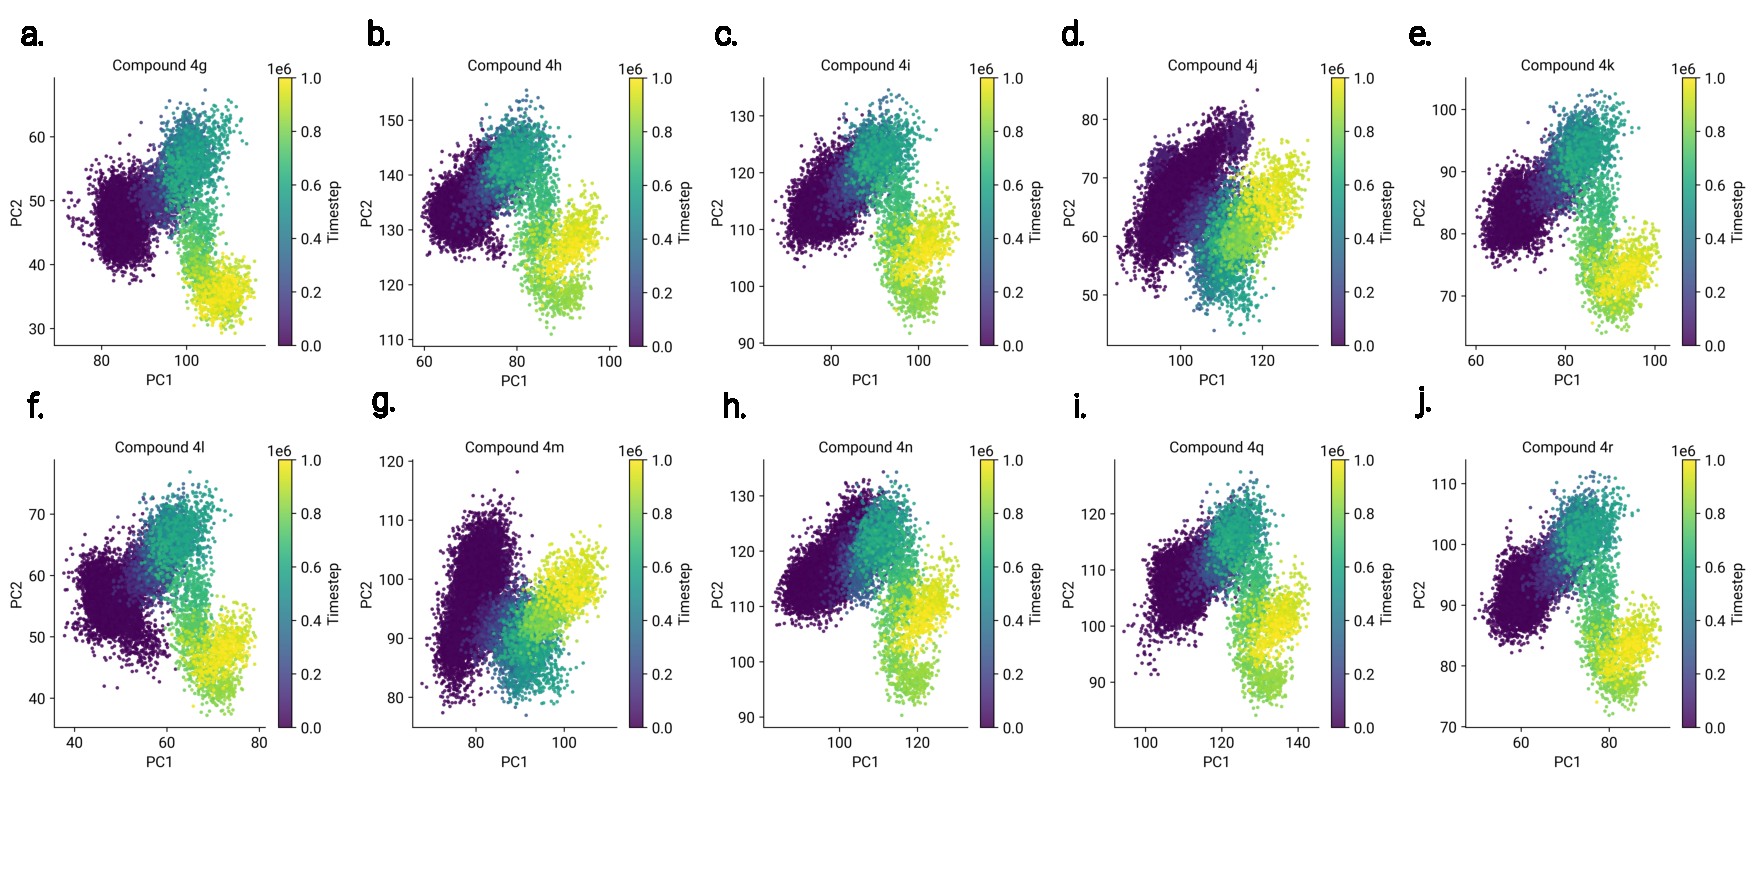
\includegraphics[width=\linewidth,height=0.68\textheight,keepaspectratio]{chapters/appendixA/figures/si_s7/si_figure_S7.pdf}
  \caption[Deflorian binding-pocket PCA coloured by simulation time.]{PCA projections of pairwise C$\alpha$ distance features, coloured by simulation time, for compounds (a) 4g, (b) 4h, (c) 4i, (d) 4j, (e) 4k, (f) 4l, (g) 4m, (h) 4n, (i) 4q, and (j) 4r. Apo simulations form a distinct cluster, with earlier apo trajectories concentrated near its centre.}
  \label{fig:si-pca-time}
  \caption*{Reproduced from SI Figure S7 of Anand et al.\cite{anand2026improving} under CC BY 4.0.}
\end{figure}
\end{landscape}

\begin{figure}[p]
  \centering
  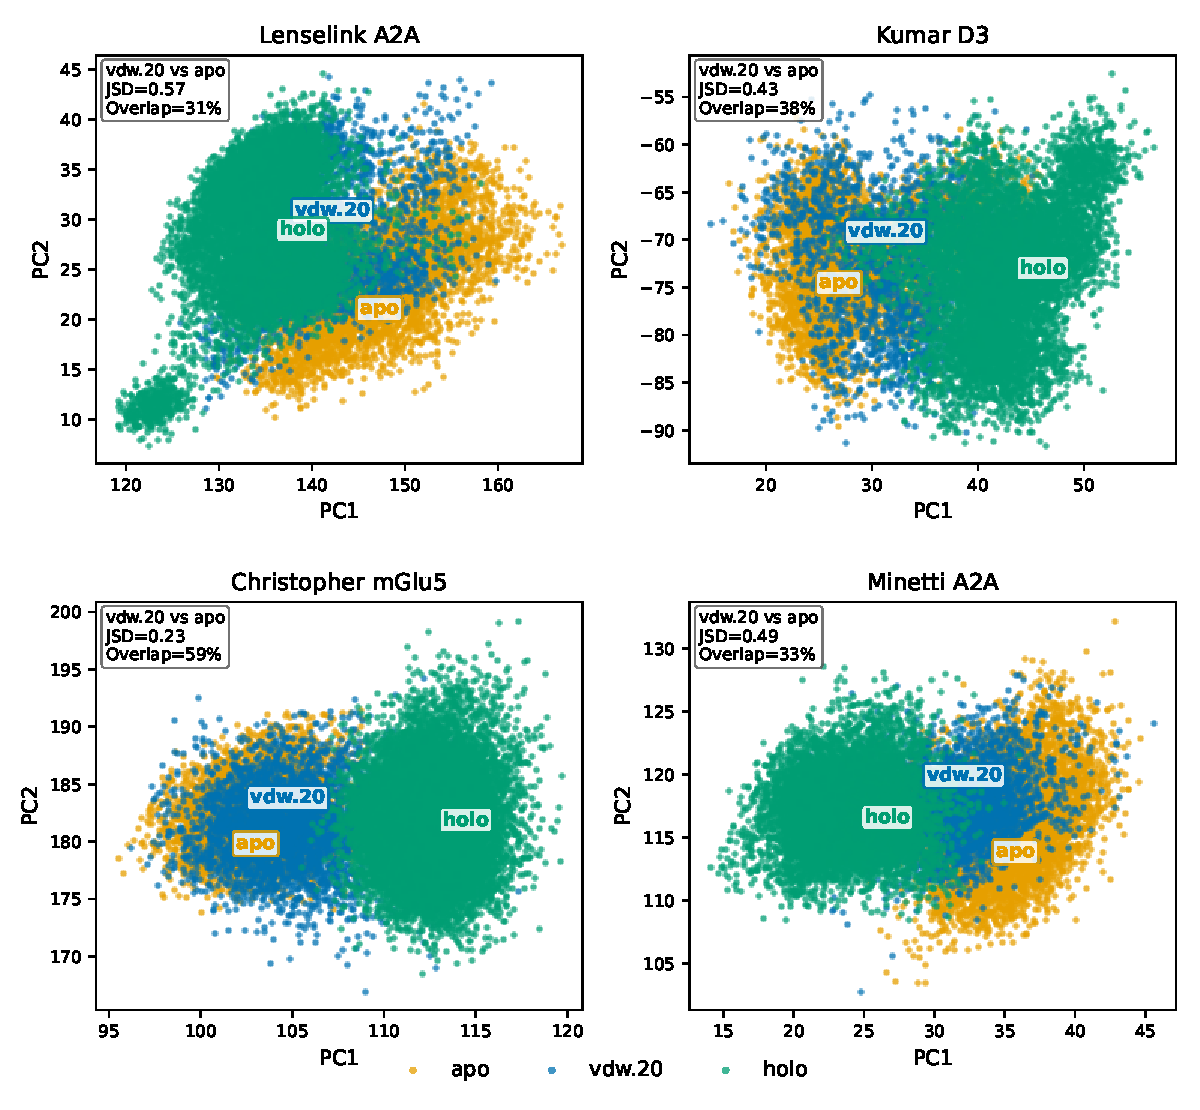
\includegraphics[width=\textwidth,height=0.66\textheight,keepaspectratio]{chapters/appendixA/figures/si_s8/si_figure_S8.pdf}
  \caption[Apo, alchemical-endpoint, and holo PCA across four datasets.]{Binding-pocket PCA comparison of apo, terminal alchemical \texttt{vdw.20}, and holo ensembles for the Lenselink A$_{2A}$, Kumar D3, Christopher mGlu5, and Minetti A$_{2A}$ datasets. Projections were generated independently from pooled ligand binding-pocket distance features. Insets compare the endpoint distribution with the apo density remaining after removing holo-overlapping density, using Jensen--Shannon divergence (JSD) and histogram overlap. Lower JSD and higher overlap indicate greater similarity.}
  \label{fig:si-pca-other-datasets}
  \caption*{Reproduced from SI Figure S8 of Anand et al.\cite{anand2026improving} under CC BY 4.0.}
\end{figure}
\clearpage

\begin{figure}[p]
  \centering
  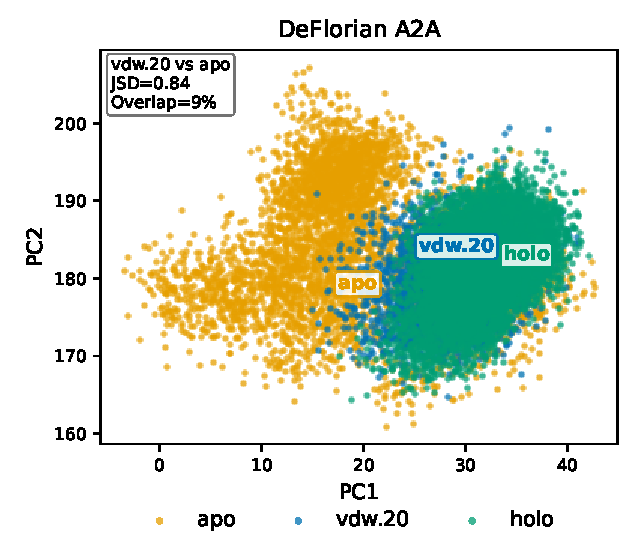
\includegraphics[width=0.86\textwidth,height=0.58\textheight,keepaspectratio]{chapters/appendixA/figures/si_s9/si_figure_S9.pdf}
  \caption[Apo, alchemical-endpoint, and holo PCA for the Deflorian dataset.]{Binding-pocket PCA comparison of apo, terminal alchemical \texttt{vdw.20}, and holo ensembles for the Deflorian A$_{2A}$ dataset. Colours identify the ensembles. The inset reports JSD and histogram overlap between the endpoint distribution and the apo density remaining after subtracting holo-overlapping density.}
  \label{fig:si-pca-deflorian-overlap}
  \caption*{Reproduced from SI Figure S9 of Anand et al.\cite{anand2026improving} under CC BY 4.0.}
\end{figure}
\clearpage

\begin{landscape}
\begin{figure}[p]
  \centering
  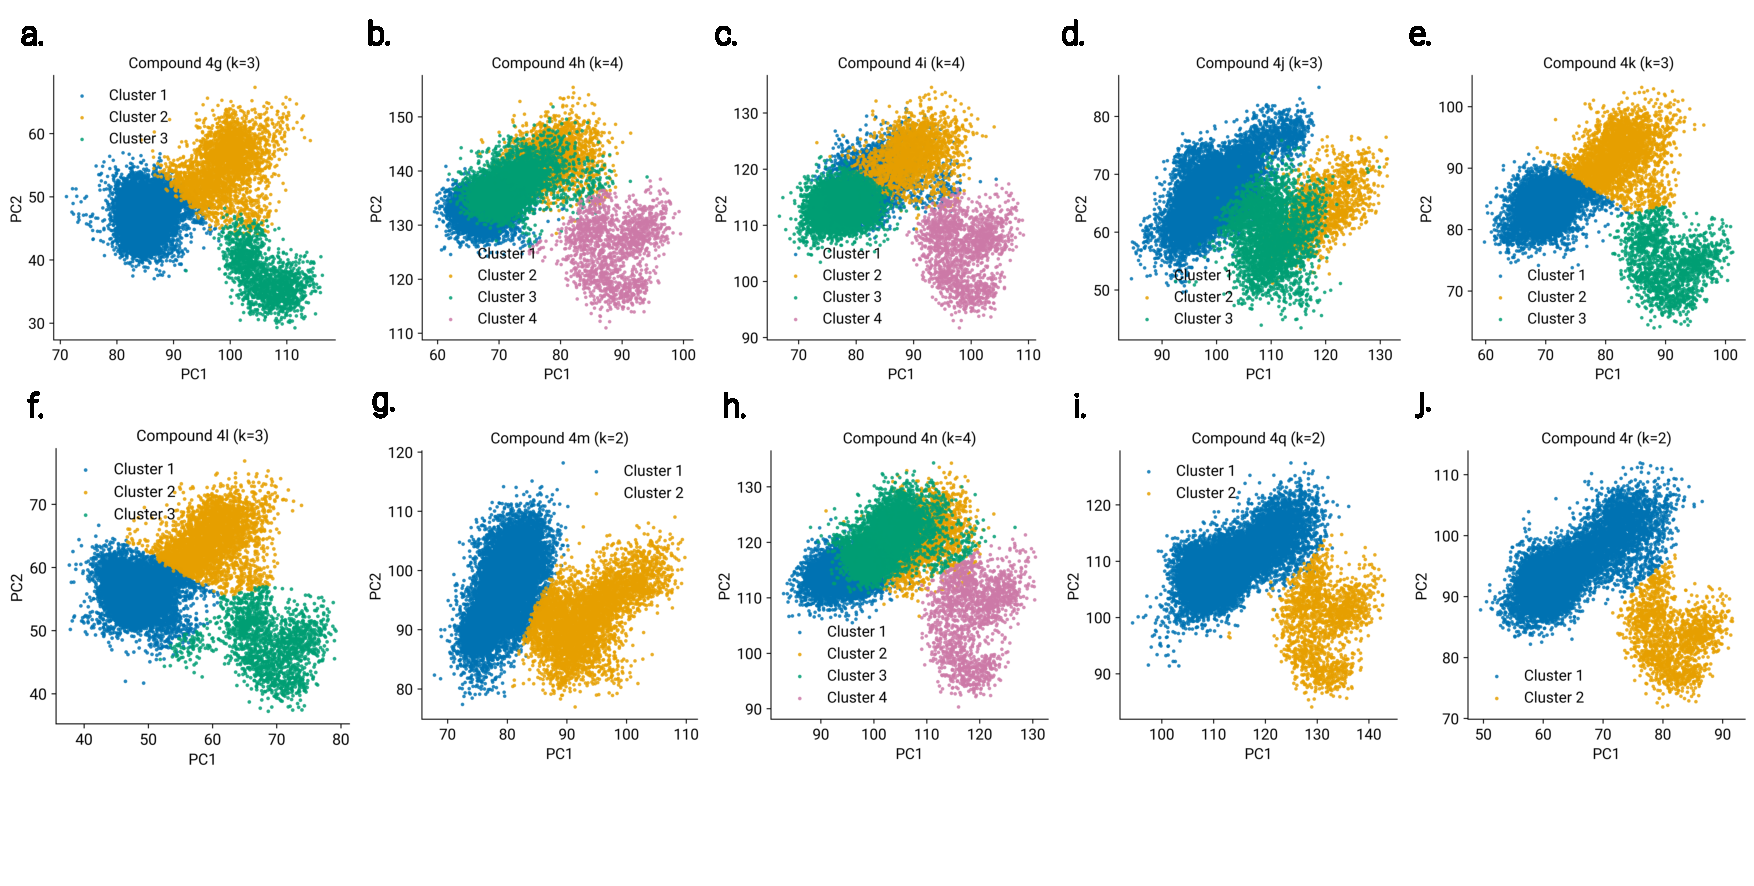
\includegraphics[width=\linewidth,height=0.66\textheight,keepaspectratio]{chapters/appendixA/figures/si_s10/si_figure_S10.pdf}
  \caption[Clustering of Deflorian binding-pocket PCA projections.]{Binding-pocket PCA projections coloured by cluster assignment for compounds (a) 4g, (b) 4h, (c) 4i, (d) 4j, (e) 4k, (f) 4l, (g) 4m, (h) 4n, (i) 4q, and (j) 4r. Two to four clusters were identified. Where several candidate apo clusters were present, the cluster with the highest proportion of apo structures was selected for REUS. Selected apo clusters were 4g: 3, 4h: 4, 4i: 4, 4j: 3, 4k: 3, 4l: 3, 4m: 2, 4n: 4, 4q: 2, and 4r: 2.}
  \label{fig:si-pca-clusters}
  \caption*{Reproduced from SI Figure S10 of Anand et al.\cite{anand2026improving} under CC BY 4.0.}
\end{figure}
\end{landscape}

\begin{landscape}
\begin{figure}[p]
  \centering
  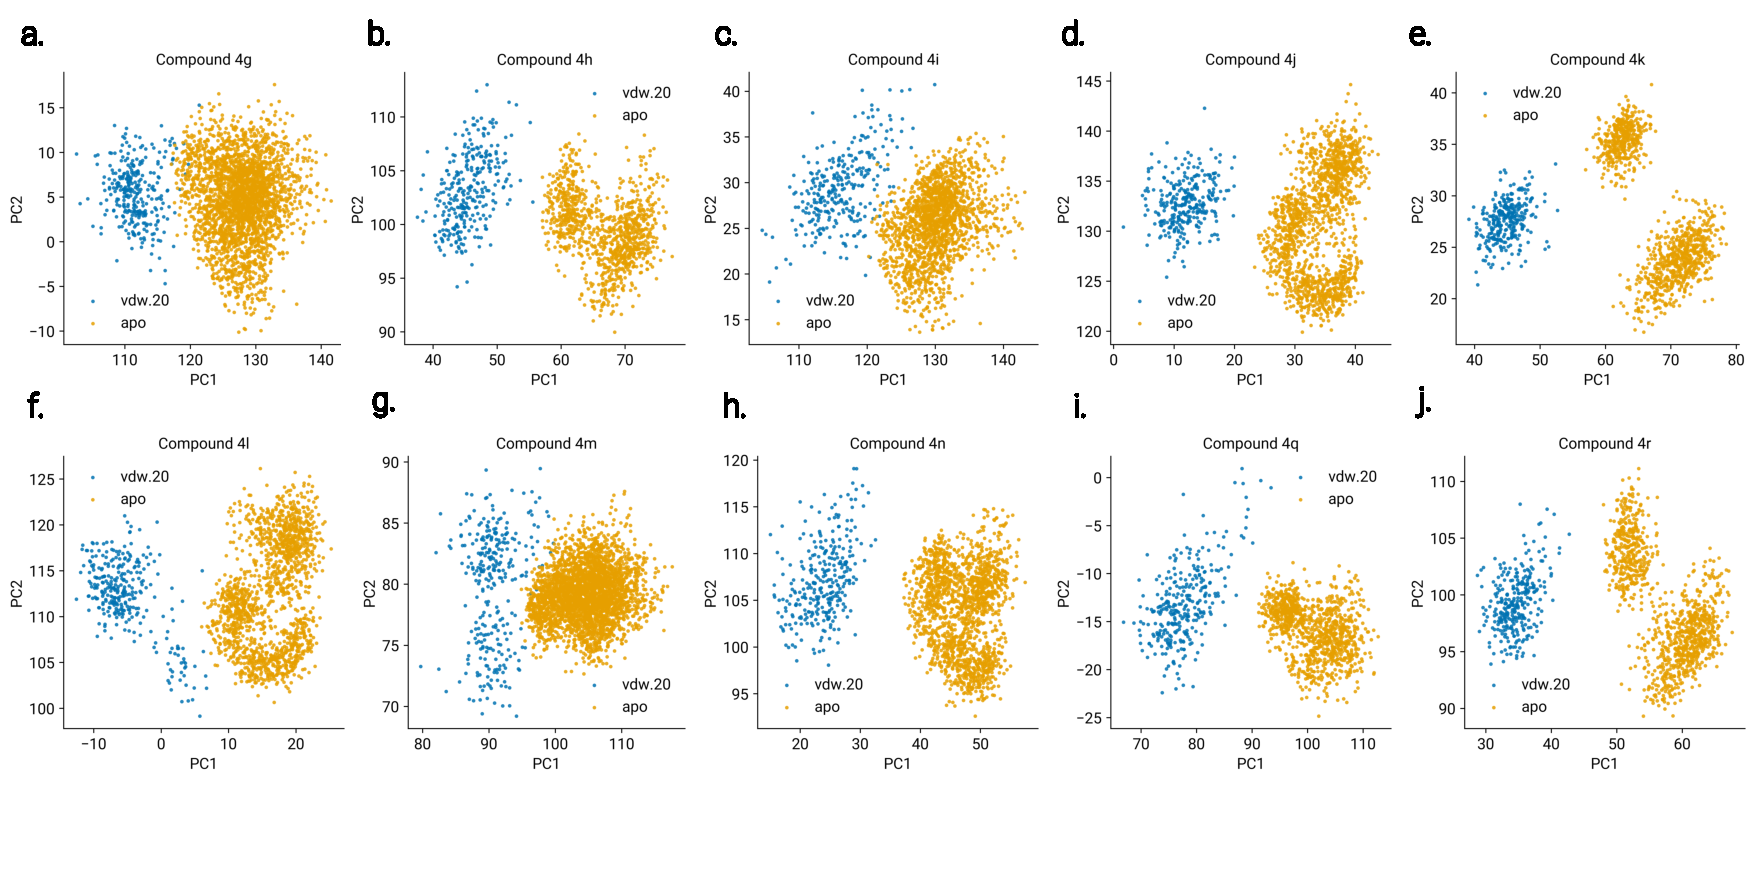
\includegraphics[width=\linewidth,height=0.68\textheight,keepaspectratio]{chapters/appendixA/figures/si_s11/si_figure_S11.pdf}
  \caption[PCA of the selected apo clusters and terminal ABFE windows.]{PCA projections of the selected apo cluster and \texttt{vdw.20} simulations for compounds (a) 4g, (b) 4h, (c) 4i, (d) 4j, (e) 4k, (f) 4l, (g) 4m, (h) 4n, (i) 4q, and (j) 4r. The first principal component of these projections defines the collective variable used for REUS.}
  \label{fig:si-pca-endpoint-cv}
  \caption*{Reproduced from SI Figure S11 of Anand et al.\cite{anand2026improving} under CC BY 4.0.}
\end{figure}
\end{landscape}

\begin{landscape}
\begin{figure}[p]
  \centering
  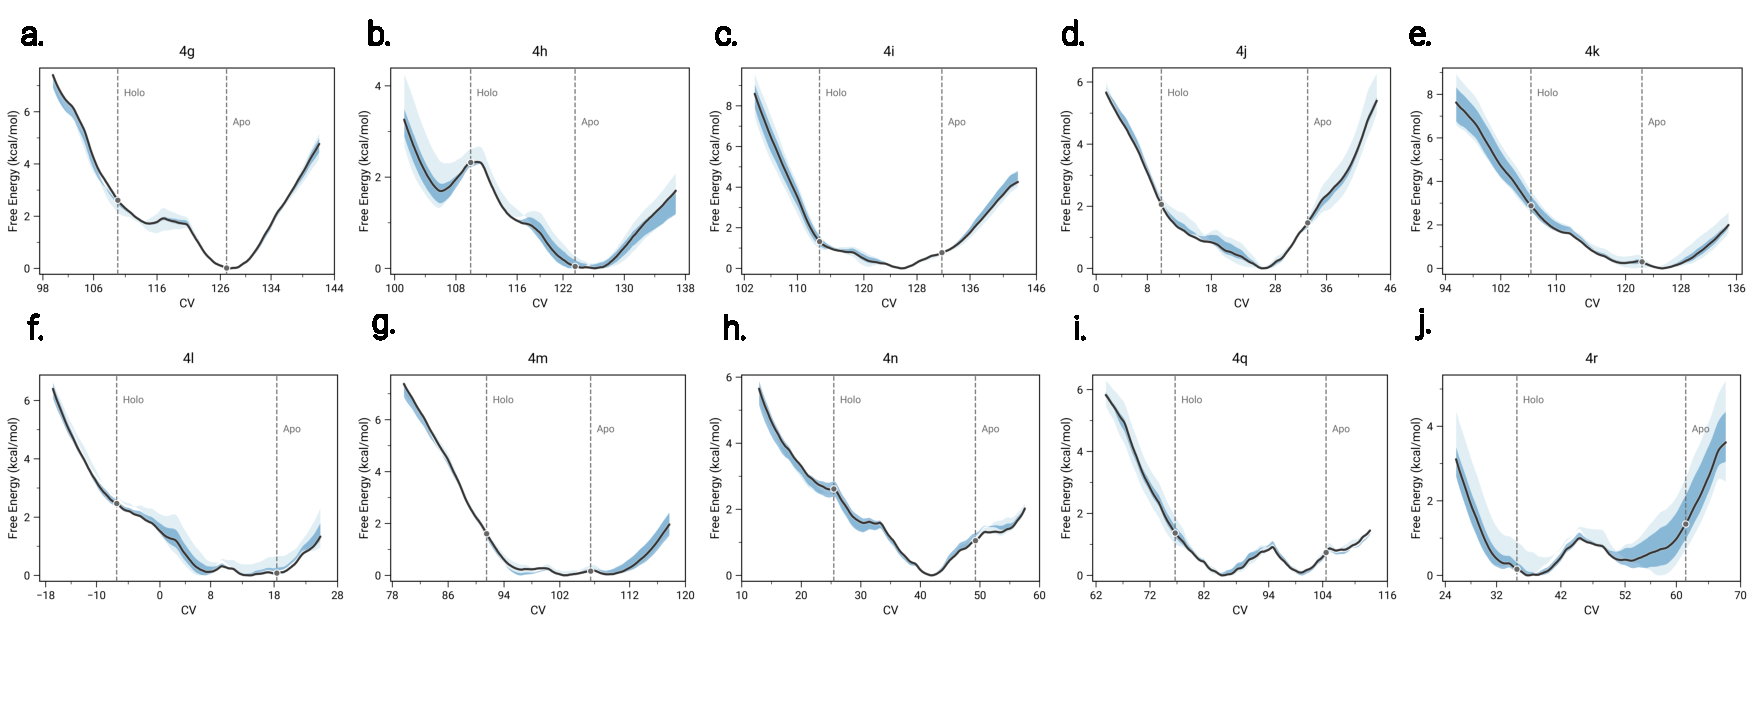
\includegraphics[width=\linewidth,height=0.68\textheight,keepaspectratio]{chapters/appendixA/figures/si_s12/si_figure_S12.pdf}
  \caption[Compound-specific REUS free-energy surfaces.]{Free-energy surfaces obtained from REUS for compounds (a) 4g, (b) 4h, (c) 4i, (d) 4j, (e) 4k, (f) 4l, (g) 4m, (h) 4n, (i) 4q, and (j) 4r. Forward and reverse profiles using different fractions of the trajectories show the convergence of the receptor relaxation estimates.}
  \label{fig:si-reus-free-energy-surfaces}
  \caption*{Reproduced from SI Figure S12 of Anand et al.\cite{anand2026improving} under CC BY 4.0.}
\end{figure}
\end{landscape}

\begin{figure}[p]
  \centering
  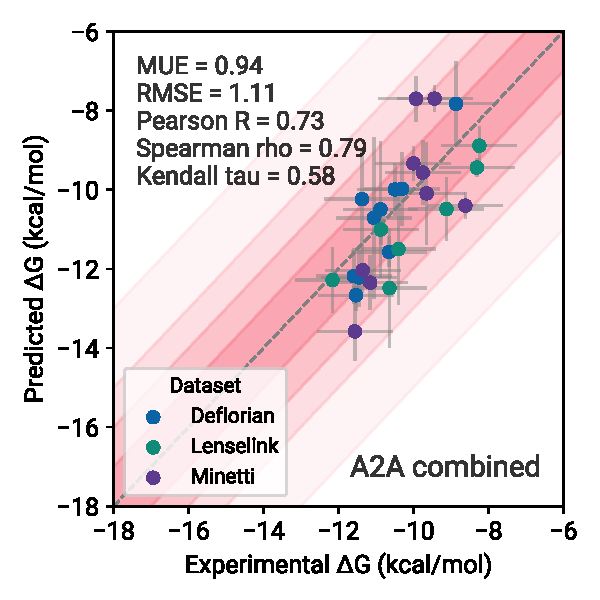
\includegraphics[width=0.82\textwidth,height=0.60\textheight,keepaspectratio]{chapters/appendixA/figures/si_s13/si_figure_S13.pdf}
  \caption[Combined A$_{2A}$ receptor ABFE performance across ligand series.]{Experimental and predicted binding free energies for the pooled Deflorian, Lenselink, and Minetti A$_{2A}$ antagonist datasets ($n=26$), coloured by source dataset. The dashed line shows perfect agreement; shaded bands indicate deviations of $1$, $2$, $3$, and $5\,\mathrm{kcal\,mol^{-1}}$. Error bars show experimental and predicted uncertainties. Statistics are calculated over the pooled dataset.}
  \label{fig:si-combined-a2a}
  \caption*{Reproduced from SI Figure S13 of Anand et al.\cite{anand2026improving} under CC BY 4.0.}
\end{figure}
\clearpage
